% arara: lualatex: {shell: 1}
%!TeX TS-program=arara
%
% This header allows you to simply invoke `arara <this-file>`
\documentclass{amsart}
\usepackage[T1]{fontenc}
%\usepackage{mathpazo}
%\usepackage[margin=1in]{geometry}
\usepackage[inline]{enumitem}
%\usepackage{rotating}
%\usepackage{color}
%\usepackage{tabu}
%\usepackage{parskip}
\usepackage{graphicx}
\usepackage{caption}
\usepackage{subcaption}
\usepackage{multicol}
\usepackage{booktabs}
\usepackage{hyperref}
\usepackage{amsmath}
\usepackage{amssymb}
\usepackage{amsthm}
\usepackage{calc}
\usepackage{xfrac}
\usepackage{mathtools}
\usepackage{cancel}
\usepackage{framed}
\usepackage{nth}
\usepackage{tikz}
\usetikzlibrary{calc,decorations.markings}
%\usepackage{xcolor-solarized}
%\usepackage{minted}
%\usepackage{MnSymbol}
%\usepackage[libertine]{newtxmath}
%\newcommand*\circled[1]{\tikz[baseline= (char.base)]{
    %\node[shape=circle,draw,inner sep=2pt] (char) {#1};}}
%\usepackage{xypic}
%\usepackage[tightpage]{preview} % display
% Math operators
\DeclareMathOperator{\Z}{\mathbb{Z}}
\DeclareMathOperator{\Q}{\mathbb{Q}}
\DeclareMathOperator{\N}{\mathbb{N}}
\DeclareMathOperator{\R}{\mathbb{R}}
\DeclareMathOperator{\C}{\mathbb{C}}
\DeclareMathOperator{\F}{\mathbb{F}}
\DeclareMathOperator{\sfe}{\mathsf{e}}
\DeclareMathOperator{\sfg}{\mathsf{g}}
\DeclareMathOperator{\sfm}{\mathsf{m}}
\DeclareMathOperator{\sft}{\mathsf{t}}
\DeclareMathOperator{\sfF}{\mathsf{F}}
\DeclareMathOperator{\sfG}{\mathsf{G}}
\DeclareMathOperator{\sfL}{\mathsf{L}}
\DeclareMathOperator{\sfP}{\mathsf{P}}
\DeclareMathOperator{\sfZ}{\mathsf{Z}}
\DeclareMathOperator{\sgAp}{Ap}
\DeclareMathOperator{\sgPF}{PF}
\DeclareMathOperator{\sgehr}{ehr}
\DeclareMathOperator{\sgconv}{conv}
\DeclareMathOperator{\sgsupp}{supp}
\DeclareMathOperator{\calC}{\mathcal{C}}
\DeclareMathOperator{\calF}{\mathcal{F}}
\DeclareMathOperator{\calO}{\mathcal{O}}
\DeclareMathOperator{\Grho}{\prescript{}{\rho}G}
% Theorem environments
\theoremstyle{plain}
\newtheorem{THM}{Theorem}
\newtheorem*{THM*}{Theorem}
\newtheorem{lemma}{Lemma}
\newtheorem*{lemma*}{Lemma}
\newtheorem*{claim}{Claim}
\newtheorem*{cor}{Corollary}
\newtheorem{prop*}{Proposition}
\newtheorem*{conj}{Conjecture}
\theoremstyle{remark}
\newtheorem*{example*}{Example}
\theoremstyle{definition}
\newtheorem*{definition*}{Definition}
% Special theorem displays
\newenvironment{thm}%
  {\begin{leftbar}\begin{THM}
}{%
  \end{THM}\end{leftbar}
}
\newenvironment{thm*}%
  {\begin{leftbar}\begin{THM*}
}{%
  \end{THM*}\end{leftbar}
}
\newenvironment{prop}%
  {\begin{leftbar}\begin{prop*}
}{%
  \end{prop*}\end{leftbar}
}
\newenvironment{definition}%
  {\begin{leftbar}\begin{definition*}
}{%
  \end{definition*}\end{leftbar}
}
\newenvironment{example}%
  {\begin{leftbar}\begin{example*}
}{%
  \end{example*}\end{leftbar}
}
% Paired math operators
\DeclarePairedDelimiter{\ceil}{\lceil}{\rceil}
\DeclarePairedDelimiter{\floor}{\lfloor}{\rfloor}
% Math helper functions
\newcommand{\congr}[2]{{[#1]}_{#2}}
\newcommand{\set}[1]{\{#1\}}
\newcommand{\genset}[1]{{\langle{}#1\rangle{}}}
\newcommand{\abs}[1]{\lvert{}#1\rvert{}}
\newcommand{\norm}[1]{\lVert{}#1\rVert{}}
\newcommand{\bmx}[1]{\begin{bmatrix}#1\end{bmatrix}}
\newcommand{\pmx}[1]{\begin{pmatrix}#1\end{pmatrix}}
  \newcommand{\sbmx}[1]{{\left[\begin{smallmatrix}#1\end{smallmatrix}\right]}}
\newcommand{\smallxymatrix}[2]{\xymatrix@C-=#1in@R-=#1in{#2}}
\renewcommand\labelitemi{\small$\bullet$}
%
%\makeatletter
\tikzset{%
  gdot/.style={draw,shape=circle,fill=black,inner sep=1},
  ddot/.style={draw,shape=circle,fill=white,inner sep=1},
  dedge/.style={draw=black!40},
  midarrow/.style={postaction={decorate},decoration={markings,mark=at position 0.5 with {\arrow{>}}}}
}
%\makeatother
\begin{document}
%
%
%

\title{Flow polytopes}
\author{Nils Olsson}
\maketitle

Based upon the book \emph{Combinatorial Reciprocity Theorems} by
Matthias Beck and Raman Sanyal; 2010 \emph{Mathematics Subject Classification}.

\hrulefill

\section*{Topic:}

\noindent
\begin{quote}
  (13) \emph{Flow polytopes.}
  A \emph{directed graph} is a collection of dots (called \emph{vertices}) and
  arrow between them (called \emph{edges}). A \emph{flow} on a directed graph is a
  way to label each edge of $G$ by an element of $\Z$ (or $\Z_n$) so that at each
  vertex $v$, the sum of the edges entering $v$ equals the sum of the edges
  leaving $v$ (i.e.\ the in \emph{flow} at each vertex equals the \emph{out
  flow}). The flows on a given directed graph can be counted using a certain
  family of polytopes, whose integer points each coincide with a flow on $G$.
  \\[1em]
  \noindent
  Source:
  \emph{Combinatorial reciprocity theorems} (M. Beck, R. Sanyal), Chapters 1 and 7.
\end{quote}

\hrulefill

\section*{Introduction}

Out of all the various topics in mathematics, graph theory is a particularly
interesting one, and is relevant to a wide variety of other mathematical
topics as well as computer science.
What this paper intends to do is, in the first section, is introduce the topic
of graphs. Many different families of graphs exist, but for this paper we will
concern ourselves with directed graphs, and $\Z_n$-flow functions which act
upon these graphs.

Then, in the second section, we will briefly explore the material of
chapter 7 of Beck and Sanyal's book \emph{Combinatorial Reciprocity Theorems},
and specifically a single main reciprocity expression theorem:
\begin{thm*}[Flow counting function]
  Let $G=(V,E)$ be a graph with a fixed base orientation.
  Then $\varphi_G(n)$ counts the number of nowhere-zero $\Z_n$-flows of $G$,
  and is defined:
  \[
    \varphi_G(n)
    =\sum_{\vec b\in\calC(G)}\sgehr_{\sfP_G^\circ(\vec b)}(n)
    ={(-1)}^{\xi(G)}\sum_{\vec b\in\calC(G)}\sgehr_{\sfP_G(\vec b)}(-n).
  \]
\end{thm*}
What this theorem provides us with is a method of traveling from the topics of
graphs and combinatorics and into the study of a seemingly unrelated
mathematical topic: polytopes.
Specifically, using polytopes to count the number of possible flows
on directed graphs, subject to a few constraints,
and even more specifically we will be looking at a way to count only the
nowhere-zero $\Z_n$-flows of a directed graph.
This should of course require a brief introduction in polytopes as well,
but as time permitted this paper wont include an introducting into polytopes or
Ehrhart reciprocity.

What this paper does \emph{not} intend to do (at least, not anymore) is
thoroughly explain the proofs of this theorem, in all of its intricacies.
Instead the second section is a restructuring of parts of chapter 7 in
Beck and Sanyal's book, in an attempt to provided a clearly progression of
concepts.

Additionally, this paper will \emph{not} work on a specific example of a graph,
as I had originally intended. I had hoped to use a very simple directed
graph to demonstrate some of the underlying mechanics of the propositions and
theorems of the book, but found it to be beyond my own scope.
%Instead, we will use a very specific and very simple example of a graph: one
%with three vertices and an edge between each pair of vertices.
%Ostensibly this forms a triangle, the simplest type of graph to which this
%theorem applies to. We will also chose a specific base orientation.
%It is with this graph that we will develop some intuition into how the main
%theorem works.
\begin{figure}[h]
  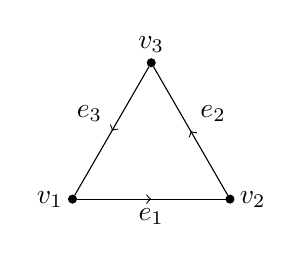
\begin{tikzpicture}
    \path[every node/.style={gdot}]
      (-1,0) node (v_1){} --
      ( 1,0) node (v_2){} --
      ($(0,{sqrt(3)})$) node (v_3){} --
      cycle;
    \node[left] at (v_1){$v_1$};
    \node[right] at (v_2){$v_2$};
    \node[above] at (v_3){$v_3$};
    \draw[midarrow] (v_1) -- node (e_1) [below]{$e_1$} (v_2);
    \draw[midarrow] (v_2) -- node (e_2) [above right]{$e_2$} (v_3);
    \draw[midarrow] (v_3) -- node (e_3) [above left]{$e_3$} (v_1);
  \end{tikzpicture}
  \caption{The intended example graph}
\end{figure}

% ------------------------------------------------------------------------------
% 1.2
% ------------------------------------------------------------------------------

\hrulefill

\section{Graphs and flows}

\subsection{Graphs}

We set off by defining and briefly explaining the topics of both graphs and
flows.
A vertex is most intuitively understood as a coordinate in space.
For instance the coordinates $x=1$ and $y=1$ can define a vertex in
Euclidean, $\R^2$, space.
An edges then is a connection between two vertices.
Edges do not necessarily need to have any particular geometric representation,
but the concept that two edges can cross over one-another will be required
later.
\begin{definition}[Graph]
  A \emph{graph} $G=(V,E)$ is a collection of $V$, a set of vertices, and $E$, a
  set of edges between the vertices.
\end{definition}

Now, a graph does not need to have any vertices.
In fact a graph with no vertices is still a graph, but it is \emph{the} empty
graph, and will not be useful in the development of the main theorem.
Nor does a graph need to have any edges (except that if a graph has edges,
then there must be vertices to which those edges connect).
Also, since a graph is just a collection of vertices and edges, we can have
graphs within graphs, i.e.\ a \emph{subgraph}, which consist of a subset of
the vertices and edges of the whole graph (in particular, every graph
necessarily has the empty graph as a subgraph, and every graph has itself as
a subgraph).

As mentioned before,
vertices, and by extension a graph, can exist within some arbitrary
d-dimensional space. However, for this report we will only concern ourselves
with graphs in two-dimensional, Euclidean space (or at least something
analogous to two dimensional).
(I will also point out that the words ``vertex'' and ``node'' are equivalent.
This paper at times switches between either word, interchangeably.)

So, given a graph with vertices and edges between vertices, we define one
classification of a subset with at least a few of its vertices, and with
possibly a few of its edges:
\begin{definition}[Component, connected component]
  A \emph{connected component} (or simply a \emph{component}) of a graph $G$ is
  a subgraph in which any two
  vertices are either directly connected via an edge, or are connected to
  one-another via a \emph{path} (a series of vertices and edges). A single
  vertex with no connecting edges is in itself a connected component.
\end{definition}

Any graph then is the disjoint union of connected components.
For example Figure~\ref{fig:disjoint-union} can be called a single graph that is the disjoint
union of three distinct connected components.
\begin{figure}[ht]
  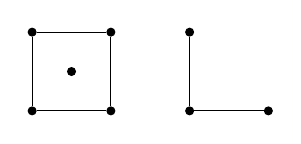
\begin{tikzpicture}[every node/.style=gdot]
    \path
      (.5,.5) node (a) {}
      (0,0) node (b) {} (1,0) node (c) {} (1,1) node (d) {} (0,1) node (e) {}
      (2,1) node (f) {} (2,0) node (g) {} (3,0) node (h) {};
    \draw (a);
    \draw (b) -- (c) -- (d) -- (e) -- (b);
    \draw (f) -- (g) -- (h);
  \end{tikzpicture}
  \caption[Disjoin union]{}\label{fig:disjoint-union}
\end{figure}
Traversing from one vertex of a graph to another by way of edges only, we see
that it may be impossible to travel to all of its vertices, hence a graph
consisting of potentially disjoint components.
\begin{lemma*}
  A connected component of the graph $G$ is a maximal subgraph of $G$ in which
  any two nodes are connect by a path.
\end{lemma*}
\begin{lemma*}
  A graph $G$ is \emph{connected} if it has only one connected component.
\end{lemma*}
\begin{definition}[Bridge]
  A \emph{bridge} is a single edge which serves as a connection between two connected
  components which, if removed, would increase the number of connected
  components of the graph by one.
\end{definition}

For example, removing the bridge in Figure~\ref{fig:bridge} turns a single
connected component into two disjoint connected components:
one complete graph into a graph with two complete subgraphs.
\begin{figure}[ht]
  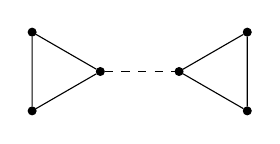
\begin{tikzpicture}[every node/.style=gdot]
    \path
      (-.5,.5) node (a) {} ($({-(1+sqrt(3))/2},0)$) node (b) {} ($({-(1+sqrt(3))/2},1)$) node (c) {}
      (.5,.5) node (d) {} ($({ (1+sqrt(3))/2},0)$) node (e) {} ($({ (1+sqrt(3))/2},1)$) node (f) {};
    \draw (a) -- (b) -- (c) -- (a);
    \draw (d) -- (e) -- (f) -- (d);
    \draw[dashed] (a) -- (d);
  \end{tikzpicture}
  \hspace{1in}
  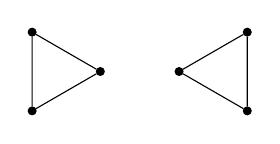
\begin{tikzpicture}[every node/.style=gdot]
    \path
      (-.5,.5) node (a) {} ($({-(1+sqrt(3))/2},0)$) node (b) {} ($({-(1+sqrt(3))/2},1)$) node (c) {}
      (.5,.5) node (d) {} ($({ (1+sqrt(3))/2},0)$) node (e) {} ($({ (1+sqrt(3))/2},1)$) node (f) {};
    \draw (a) -- (b) -- (c) -- (a);
    \draw (d) -- (e) -- (f) -- (d);
  \end{tikzpicture}
  \caption[Bridges]{An undirected graph
  with and without a bridge.}\label{fig:bridge}
\end{figure}

\subsection{Directed graphs}

So far we've only looked at \emph{unoriented} graphs, but
now we introduce a notion of direction, or orientation, to graphs.
\begin{definition}[Directed, oriented graph]
  A \emph{directed} or \emph{oriented graph} is a graph on which we
  define an \emph{orientation} via a subset $\rho$ of the edges $E$ of the
  graph. For each edge $e=v_i v_j\in E$ (connecting the vertices $v_i,v_j\in
  V$) with $i<j$ we direct:
  \[
    v_i\stackrel{e}{\leftarrow}v_j\text{ if }e\in\rho\text{, and }
    v_i\stackrel{e}{\rightarrow}v_j\text{ if }e\notin\rho.
  \]
  The graph $G$ with orientation $\rho$ is denoted ${}_\rho G$.
\end{definition}
This definition may be confusing at first glance because $\rho$
may be missing some of the edges of $E$. It only includes the edges with
their direction pointing from the vertex of higher index to the vertex of lower
index (which does certainly feel backwards).
Then, all of the edges not in $\rho$ are directed in the opposite
direction: from lower to higher index.

Figure~\ref{fig:directed-graph} demonstrate how this encapsulation works by
applying an orientation $\rho=\{14,23,24\}$ onto a particular graph in three
steps.
\begin{figure}[ht]
  \begin{subfigure}[t]{0.3\textwidth}
    \centering
    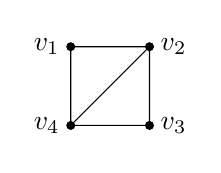
\begin{tikzpicture}[every node/.style=gdot]
      \path
        (0,1) node (v_1)[label=left:$v_1$]{}
        (1,1) node (v_2)[label=right:$v_2$]{}
        (1,0) node (v_3)[label=right:$v_3$]{}
        (0,0) node (v_4)[label=left:$v_4$]{};
      \draw (v_4) -- (v_3) -- (v_2) -- (v_1) -- (v_4) -- (v_2);
    \end{tikzpicture}
    \caption{The undirected graph.}
  \end{subfigure}
  %\hspace{1in}
  \begin{subfigure}[t]{0.3\textwidth}
    \centering
    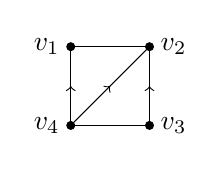
\begin{tikzpicture}[every node/.style=gdot]
      \path
        (0,1) node (v_1)[label=left:$v_1$]{}
        (1,1) node (v_2)[label=right:$v_2$]{}
        (1,0) node (v_3)[label=right:$v_3$]{}
        (0,0) node (v_4)[label=left:$v_4$]{};
      \draw[midarrow] (v_4) -- (v_1);
      \draw[midarrow] (v_4) -- (v_2);
      \draw[midarrow] (v_3) -- (v_2);
      \draw (v_3) -- (v_4);
      \draw (v_1) -- (v_2);
    \end{tikzpicture}
    \caption{$\rho$ edges marked.}
  \end{subfigure}
  \begin{subfigure}[t]{0.3\textwidth}
    \centering
    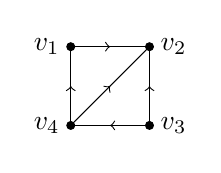
\begin{tikzpicture}[every node/.style={gdot}]
      \path
        (0,1) node (v_1)[label=left:$v_1$]{}
        (1,1) node (v_2)[label=right:$v_2$]{}
        (1,0) node (v_3)[label=right:$v_3$]{}
        (0,0) node (v_4)[label=left:$v_4$]{};
      \draw[midarrow] (v_4) -- (v_1);
      \draw[midarrow] (v_4) -- (v_2);
      \draw[midarrow] (v_3) -- (v_2);
      \draw[midarrow] (v_3) -- (v_4);
      \draw[midarrow] (v_1) -- (v_2);
    \end{tikzpicture}
    \caption{$E\setminus\rho$ edges marked.}
  \end{subfigure}
  \caption[A directed graph]{A directed graph.}\label{fig:directed-graph}
\end{figure}

As an aside, there are many algorithms in computer science pertaining to graphs,
some for finding optimal ways to traverse the paths of graphs. In some
models each edge is considered to be of equal ``weight'' to any
other. That is, if two unweighted edges both originate from a node $v_1$
and both point to a second node $v_2$, then there is no reason to choose one
edge over the other in traveling from $v_1$ to $v_2$.
On the other hand, we might assign a weight to
each edge, presenting a cost-benefit analysis in choosing a path to take (as in
Figure~\ref{fig:path-finding}, where the edge with weight 5 now becomes most
``expensive'' to traverse versus the one with weight 2).
\begin{figure}[ht]
  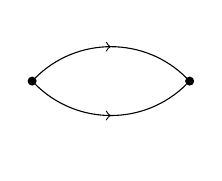
\begin{tikzpicture}
    \path (0,0) node[gdot] (a){} (2,0) node[gdot] (b){};
    \draw[midarrow] (a) to [out=45, in=135] node[above]{} (b);
    \draw[midarrow] (a) to [out=315,in=225] node[below]{$\phantom 5$} (b);
  \end{tikzpicture}
  \hspace{1in}
  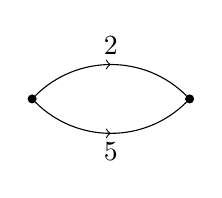
\begin{tikzpicture}
    \path (0,0) node[gdot] (a){} (2,0) node[gdot] (b){};
    \draw[midarrow] (a) to [out=45, in=135] node[above]{$2$} (b);
    \draw[midarrow] (a) to [out=315,in=225] node[below]{$5$} (b);
  \end{tikzpicture}
  \caption{A directed graph, with and without weights.}\label{fig:path-finding}
\end{figure}

\begin{definition}[Directed path, directed cycle]
  A \emph{directed path} in ${}_\rho G$ is a sequence $v_0,v_1,\ldots,v_s$ of
  distinct nodes such that $v_{j-1}\to v_j$ is a directed edge in ${}_\rho G$
  for all $j=1,\ldots,s$. If $v_s\to v_0$ is also a directed edge, then
  $v_0,v_1,\ldots,v_s,v_{s+1}=v_0$ is called a \emph{directed cycle}.
\end{definition}

\begin{definition}[Acyclic orientations]
  An orientation $\rho$ of $G$ is acyclic if there are no directed cycles in
  ${}_\rho G$.
\end{definition}

Dual to the notion of acyclic orientations are orientations which are
\emph{totally cyclic}, where every edge in ${}_\rho G$ is contained in a
directed cycle.
\begin{figure}[h]
  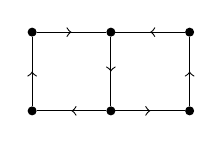
\begin{tikzpicture}
    \path[every node/.style={gdot}]
      (-1, 0) node(a){} --
      (-1, 1) node(b){} --
      ( 0, 1) node(c){} --
      ( 0, 0) node(d){} --
      ( 1, 0) node(e){} --
      ( 1, 1) node(f){};
    \draw[midarrow] (c) -- (d);
    \draw[midarrow] (a) -- (b);
    \draw[midarrow] (b) -- (c);
    \draw[midarrow] (d) -- (a);
    \draw[midarrow] (e) -- (f);
    \draw[midarrow] (f) -- (c);
    \draw[midarrow] (d) -- (e);
  \end{tikzpicture}
  \caption{A totally cyclic graph with two cycles.}
\end{figure}

\begin{definition}[Cyclotomic number]
  We define the \emph{cyclotomic number} of $G$ as:
  \[
    \xi(G)=|E|-|V|+c.
  \]
  Where $c=c(G)$ is the number of connected components of $G$.
\end{definition}

Another topic of graphs is coloring, where every vertex is assigned a color
value, and a proper coloring is where no vertices connected by an edge share the
same color. Directions and cycles provide a particular way to induce a coloring
onto the vertices of a graph, but this is outside the scope of this paper.
However, acyclic and cyclic orientations are a critical component of
the main focus of this paper, the nowhere-zero $\Z_n$-flow counting function,
which we now introduce.

\subsection{Flows}

With a notion of orientations and weights upon the edges of graphs,
we will now introduce a particular type of weight value that is specific to
living within an Abelian group $\Z_n=\sfrac\Z n$, and a function which gives
to every edge of a graph this particular type of weight:
%(There may also be optimal path algorithms associated
%with flow values, similar to weights on directed edges, but for this paper our
%focus is elsewhere.)
\begin{definition}[$\Z_n$-flow]
  A \emph{$\Z_n$-flow} is a map $f:E\to\Z_n$ which to each edge, $e$, of a
  directed graph assigns a flow value, ${f(e)\in\Z_n}$, such that there is
  ``conservation of flow'' at every vertex, $v$, by which me mean the sum of the
  flows into a vertex is congruent to the sum of the flows out it:
  \[
    \sum_{\stackrel e \to v}f(e)=\sum_{v\stackrel e \to}f(e).
  \]
\end{definition}

It is these flow functions that are the subject of the main theorem of this
paper, in particular counting how many different flows can be constructed for
a particular directed graph given the constraint of conservation.
It is especially important to note that because the flow values are elements of
an Abelian group $\Z_n$ that there is necessarily a finite number of flow
functions that can be applied to any particular graph since each flow value
has to be one of $n$ possible values, modulus $n$.

\begin{definition}[$f$ support]
  The \emph{support} of $f$, denoted $\sgsupp(f)$, is the subset of edges $e$
  whose flows are non-zero:
  \[
    \sgsupp(f)=\{e\in E:f(e)\ne 0\}\subseteq E
  \]
\end{definition}
If $\sgsupp(f)=E$ (all $e$ edges have $f(e)\ne0$), then $f$ is considered
``nowhere-zero''. For the rest of this report we'll be concerned with these
nowhere-zero $\Z_n$-flows, in particular with counting how many of them can be
made for any particular graph and Abelian group.
%
Figure~\ref{fig:graph-flows} illustrates two different but satisfactory
$\Z_5$-flows on a graph.
As simple integer weights, the second flow would not fullfil the conservation
requirement, since from vertex $v_1$ we have in input of 0 and an output of
$2+3=5$,
but as elements of the Abelian group $Z_5$ they work, since
$5\equiv 0\bmod 5$.
\begin{figure}[ht]
  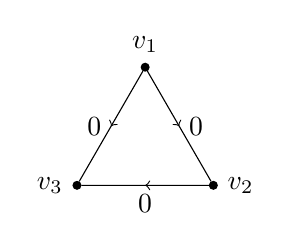
\begin{tikzpicture}
    \path
      (0,1) node (a)[gdot,label=$v_1$]{}
      ($({cos(  -pi/6 r)},{sin(  -pi/6 r)})$) node (b)[gdot,label=right:$v_2$]{}
      ($({cos(-5*pi/6 r)},{sin(-5*pi/6 r)})$) node (c)[gdot,label=left:$v_3$]{};
    \draw[midarrow] (a) -- node[right]{0} (b);
    \draw[midarrow] (a) -- node[left]{0} (c);
    \draw[midarrow] (b) -- node[below]{0} (c);
  \end{tikzpicture}
  \hspace{1in}
  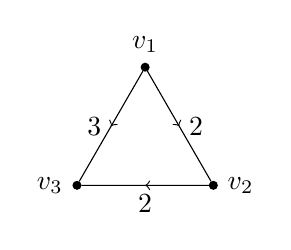
\begin{tikzpicture}
    \path
      (0,1) node (a)[gdot,label=$v_1$]{}
      ($({cos(  -pi/6 r)},{sin(  -pi/6 r)})$) node (b)[gdot,label=right:$v_2$]{}
      ($({cos(-5*pi/6 r)},{sin(-5*pi/6 r)})$) node (c)[gdot,label=left:$v_3$]{};
    \draw[midarrow] (a) -- node[right]{2} (b);
    \draw[midarrow] (a) -- node[left]{3} (c);
    \draw[midarrow] (b) -- node[below]{2} (c);
  \end{tikzpicture}
  \caption{An everywhere-zero $\Z_5$-flow and a nowhere-zero $\Z_5$-flow.}\label{fig:graph-flows}
\end{figure}

%Going forward, $G$ will always refer to a 2-dimensional graph with $V$ vertices
%and $E$ edges, $\rho$ to an arbitrary  orientation of $G$
%and $\Z_n$ to an Abelian group to which $f$ a $\Z_n$-flow maps.
And now we introduce the main focus of this paper.
\begin{definition}[Nowhere-zero $\Z_n$-flow counting function]
  Define a counting function:
  \[
    \varphi_G(n)=\text{the number of $f$ nowhere-zero $\Z_n$-flows on $G$}
  \]
\end{definition}
As it happens\ldots
\begin{prop}
  The flow-counting function $\varphi_G(n)$ is independent of the orientation
  $\rho$ of $G$.
\end{prop}
\begin{prop}
  $G$ will not have any nowhere-zero flow if $G$ has a \emph{bridge}---an edge
  whose removal increases the number of connected components of $G$.
\end{prop}

\subsection{Dual graphs}

Consider a graph $G$ as subdividing the plane into connected regions. If two
points lie within a region then they can be connected without intersecting an
edge of $G$. Regions which are neighbors have an edge of $G$ which separate them
(their topological closures sharing a proper 1-dimensional part of their
boundaries).
\begin{definition}[Dual graph]
  The \emph{dual graph} of a graph $G=(V,E)$ is the graph $G^*=(V^*,E^*)$ with
  vertices corresponding to the regions of $G$.
  %
  Two vertices $u^*,v^*\in V^*$
  which correspond to two regions $R_{u^*}$ and $R_{v^*}$ of $G$ are connected via edge $e^*\in
  E^*$ if an original edge $e\in E$ is properly contained within the boundaries
  of $R_{u^*}$ and $R_{v^*}$.
\end{definition}
%Figure~\ref{fig:dual-incomplete} shows a graph with four vertices (solid)
%along with the vertices (hollow) of its dual to demonstrate the regions which
%$G$ subdivides the plane into.
%(However the edges are omitted.
%See Figure~\ref{fig:graphs-and-duals} for complete illustrations of graphs and
%their duals.)
%\begin{figure}[ht]
    %\begin{tikzpicture}
      %\path
        %(0,0) node (a)[gdot]{}
        %(1,0) node (b)[gdot]{}
        %(1,1) node (c)[gdot]{}
        %(0,1) node (d)[gdot]{};
      %\draw (a) -- (b) -- (c) -- (d) -- (a);
      %\path (.5,.5) node[ddot]{} (1.5,.5) node[ddot]{};
  %\end{tikzpicture}
  %\caption{A graph and its (incompletely portrayed) dual graph.}
  %\label{fig:dual-incomplete}
%\end{figure}
In other words there is one $e^*$ for
every edge $e$ that lies between two regions of $G$; it connects the $G^*$
vertices corresponding to the two regions; and it crosses over its
corresponding $e$ edge ($e$ and $e^*$ intersect).
%
But as a single illustration says a thousand words,
Figure~\ref{fig:graphs-and-duals} illustrates a few examples of graphs
(solid dot vertices) and their duals (hollow dot vertices).
\begin{figure}[ht]
  \begin{subfigure}[t]{.3\textwidth}
    \begin{tikzpicture}[
        gdot/.style={draw,shape=circle,fill=black,inner sep=1},
        ddot/.style={draw,shape=circle,fill=white,inner sep=1},
        decoration={markings,mark=at position 0.5 with {\arrow{>}}}
      ]
      \begin{scope}
        %\clip (-2,-1) rectangle (2,2);
        \draw (0,0) node[gdot](a){} -- (1,0) node[gdot](b){};
        \node[ddot](c) at (.5,-.5) {};
        \draw[dedge] (c) to [out=180,in=90,looseness=60] (c);
      \end{scope}
    \end{tikzpicture}
    \caption{Simplest graph with a bridge.}
  \end{subfigure}
  %\begin{subfigure}[t]{.3\textwidth}
    %\begin{tikzpicture}[
        %gdot/.style={draw,shape=circle,fill=black,inner sep=1},
        %ddot/.style={draw,shape=circle,fill=white,inner sep=1},
        %decoration={markings,mark=at position 0.5 with {\arrow{>}}}
      %]
      %\begin{scope}
        %%\clip (-2,-1) rectangle (2,2);
        %\draw (0,0) node[gdot]{} -- (1,0) node[gdot]{} -- ($(1/2,{sqrt(3)/2})$) node [gdot]{} -- cycle;
        %\node[ddot] (a) at ($(1/2,{-sqrt(2)/3})$) {};
        %\node[ddot] (b) at ($(1/2,{sqrt(3)/6})$) {};
        %\draw[dedge] (a) -- (b);
        %\draw[dedge] (a) to [out=180,in=135,looseness=4] (b);
        %\draw[dedge] (a) to [out=0,in=45,looseness=4] (b);
      %\end{scope}
    %\end{tikzpicture}
    %\caption{A complete graph.}
  %\end{subfigure}
  %\begin{subfigure}[t]{.3\textwidth}
    %\begin{tikzpicture}[
      %gdot/.style={draw,shape=circle,fill=black,inner sep=1},
      %ddot/.style={draw,shape=circle,fill=white,inner sep=1},
      %decoration={markings,mark=at position 0.5 with {\arrow{>}}}
    %]
    %\begin{scope}
      %%\clip (-2,-1) rectangle (2,2);
      %\draw (0,0) node[gdot]{} -- (0,1) node[gdot]{};
      %\draw (0,0) node[gdot]{} -- ($({sqrt(3)/2},1/2)$) node[gdot]{} -- (0,1) node[gdot]{} -- ($({-sqrt(3)/2},1/2)$) node[gdot]{} -- cycle;
      %\node[ddot] (a) at (0,-1/2){};
      %\node[ddot] (b) at ($({-sqrt(3)/6},1/2)$){};
      %\node[ddot] (c) at ($({ sqrt(3)/6},1/2)$){};
      %\draw[dedge] (a) to [out=120,in=240] (b);
      %\draw[dedge] (a) to [out=180,in=120,looseness=4] (b);
      %\draw[dedge] (a) to [out=60,in=300] (c);
      %\draw[dedge] (a) to [out=0,in=60,looseness=4] (c);
      %\draw[dedge] (b) -- (c);
    %\end{scope}
    %\end{tikzpicture}
    %\caption{Graph with two connected components.}
  %\end{subfigure}
  \caption{Various graphs and their duals.}\label{fig:graphs-and-duals}
\end{figure}

What naturally follows is that if $G$ is a directed graph, we should want
$G^*$ to also be some sort of directed graph.
So, given an orientation of $G$, an orientation on $G^*$ can be induced by
``rotating'' the direction of the edge clockwise. That is, the dual edge $e^*$
will ``point'' east assuming that the primal edge $e$ points north.
%\begin{figure}[ht]
%\begin{tikzpicture}
%\draw[->,thick] (.25,0) .. controls (.25,.5) and (.75,.5) .. (.75,1);
%\draw[->,dedge] (0,.5) -- (1,.5);
%\end{tikzpicture}
%\hspace{1in}
%\begin{tikzpicture}
%\draw[<-,thick] (.25,0) .. controls (.25,.5) and (.75,.5) .. (.75,1);
%\draw[<-,dedge] (0,.5) -- (1,.5);
%\end{tikzpicture}
%\end{figure}

% ------------------------------------------------------------------------------
% 7.6
% ------------------------------------------------------------------------------
\hrulefill

\section{Reciprocity in counting nowhere-zero $\Z_n$-flows}

Originally my intention of this second section of the paper was to demonstrate,
by example, the underlying mechanisms of the theorems and propositions in the
Beck and Sanyal book. Instead what I found was that my grasp on the topic was
shaky at best. What proved the most useful, to me at least, was to piece
together a different order of the book's chapter 7 definitions, propositions and
theorems; an order which feels much more natural in moving from a graph and
combinatorial centric topic of flows, into a more polytope centric topic of
reciprocity expressions.
It was also at this time that I recognized that many topic introduced in the
first second of this paper would now have no connection to this second section,
specifically dual graphs and cyclic/acyclic orientations.
They are in fact critical in the proofs of the propositions behind the
$\Z_n$-flow counting function, but by limitations of time wont find any use
here-on-out.

%Instead of regurgitate the general proof of the main theorem, in this section we
%will observe the mechanics of the theorem by studying a specific directed graph
%with vertices $V=\{v_1,v_2,v_3\}$,
%edges $E=\{e_1=v_1v_2,e_2=v_2v_3,e_3=v_3v_1\}$, and
%base orientation $\rho=\{21,32,31\}$.
%\begin{figure}[h]
  %\begin{tikzpicture}
    %\path[every node/.style={gdot}]
      %(-1,0) node (v_1){} --
      %( 1,0) node (v_2){} --
      %($(0,{sqrt(3)})$) node (v_3){} --
      %cycle;
    %\node[left] at (v_1){$v_1$};
    %\node[right] at (v_2){$v_2$};
    %\node[above] at (v_3){$v_3$};
    %\draw[midarrow] (v_1) -- node (e_1) [below]{$e_1$} (v_2);
    %\draw[midarrow] (v_2) -- node (e_2) [above right]{$e_2$} (v_3);
    %\draw[midarrow] (v_3) -- node (e_3) [above left]{$e_3$} (v_1);
  %\end{tikzpicture}
  %\caption{Our graph, $G=(V,E)$.}\label{fig:our_graph}
%\end{figure}
%We choose this graph in particular for its simplicity. It is (I believe) the
%simplest example of a bridgeless, connected, and totally cyclic graph.

We begin by recalling that flows are functions which assign to every edge of a
directed graph a value such that there is conservation of flow at every vertex:
\[
  \sum_{u\rightarrow v}f(uv)-\sum_{u\leftarrow v}f(uv)=0.
\]
What may not be obvious from the presentation of this equation is that it is
specific to the vertex $v$ and not to $u$. Rather, $u$ pertains to the other
side of an edge, pointing towards $v$ or away from it; there may be many
different $u$ vertices, depending on how many edges connect to a particular $v$.

We will also pay attention to the specific order of the vertices in $V$ and the
specific order of the edges in $E$.
What this provides us with is a way to think of flow functions as coordinates,
where each flow value is a component of a $m$-dimensional coordinate,
indexed by the edge onto which it is assigned:
\[
  f=(f(e_1),f(e_2),\ldots,f(e_m)).
\]
This is extremely important, as it allows us to eventually build polytopes
from collections of possible flows.

%(Note that the source paper introduces flows as being real-valued, but I will
%gloss over this as it is real-valued flows are really only necessary in the
%proof of various propositions.)

Also recall that $\Z_n$-flows (a specific kind of flow function)
assign to edges flow values which are elements of an Abelian group $\Z_n$.
The conservation equation then is modified to look more like the remainder
algorithm:
\begin{equation}
  \sum_{u\rightarrow v}f(uv)-\sum_{u\leftarrow v}f(uv)=nb_v.\label{eqn:flow_conservation}
\end{equation}
Where $b_v$ is an integer, and each $b_v$ corresponds to a specific vertex $v$
of our graph. That is, $b_1$ corresponds to $v_1$, $b_2$ to $v_2$,
and $b_3$ to $v_3$.
We will collect these $b_v$ values into a vector $\vec b=(b_1,b_2,b_3)\in \Z^V$
in order of the vertices,
just as we considered the order of the edges in calling a flow $f$ a
coordinate.

We should note that the $\Z_n$-flows, $f\in\Z_n^E$, are just one particular
solution to this inequality (it's actually surprising to me that the book never
uses the notation $\Z_n^E$ for flow values corresponding to the vertices). Many
more solutions may exist, in particular for real-valued flows, $f\in\R^E$.
Certainly it is confusing having the symbol $f$ change family like this, and the
book makes little-to-no distinction.
%
Even so, for $\vec b\in\Z^V$ we define the following:
\begin{definition}[Subspace of flows]
  Let $G=(V,E)$ be a graph with a fixed base orientation.
  We define $\calF(\vec b)\subseteq\R^E$ to be the
  affine subspace of all $f\in\R^E$ real-valued flows
  (also considering $f$ as a real-valued coordinate)
  satisfying~\eqref{eqn:flow_conservation} when $n=1$.
\end{definition}

Moving towards our goal, the number of nowhere-zero $\Z_n$-flows of $G$,
$\varphi_G(n)$, then (hinting to polytopes) is the number of lattice points in
\[
  n{(0,1)}^E\cap\bigcup_{\vec b\in\Z^V}\calF_G(n\vec b).
\]
However this collection contains much more than just the lattice points,
since $\calF_G(n\vec b)$ contains all real-valued flows.

Another important property of the flow subspaces to note is when
$\vec b=\vec 0$. In fact we give this particular subspace its own definition:
\begin{definition}[Flow space]
  Let $G=(V,E)$ be a graph with a fixed base orientation.
  We call $\calF_G(\vec 0)$ the \emph{flow space} of $G$, and simply
  denote it $\calF_G$.
\end{definition}
Notice that, for the flow space, equation~\eqref{eqn:flow_conservation} turns
into an inequality:
\[
  \sum_{u\rightarrow v}f(uv)=\sum_{u\leftarrow v}f(uv).
\] 
This condition is called the \emph{conservation of flow} at every $v$,
hearkening back to the original definition of weights and flows, in the first
section of this paper.
An important takeaway from this fact is that for any $\vec b\in\Z^E$,
$\calF_G(\vec b)=t+\calF_G(\vec 0)$
for some $t\in\R^E$, meaning that the dimension of the flow subspace
$\calF_G(\vec b)$ (not to be confused with the flow space $\calF$)
is actually independent of $\vec b$.
As I wont be including any of the proofs of the book in the paper, the following
proposition may not be obvious.
\begin{prop}
  Let $G=(V,E)$ be a graph with a fixed base orientation.
  Then the dimension of the flow space $\dim\calF_G=\xi(G)$.
\end{prop}
But what this proposition hints at is the relation between cycles in a graph
and the flow space (recall that $\xi(G)$ is the cyclotomic number of a graph
$G$).

Going back to the $\vec b$ vectors,
we make the following set definition by recognizing that although many of the
$\vec b$ vectors may satisfy equation~\eqref{eqn:flow_conservation}, many
still may be somewhere-zero flows:
\begin{definition}[Nowhere-zero flow vectors]
  Let $\calC(G)\subset\Z^V$ be the set of all $\vec b$ vectors such that:
  \[
    {(0,1)}^E\cap\calF_G(\vec b)\ne\emptyset.
  \] 
\end{definition}
The book makes no name for this set, but we will refer to it as the nowhere-zero
flow vector set.

\hrulefill

Finally we are ready move into the world of polytopes proper.
In particular we can start to see
that the polytope we are constructing
will have vertices corresponding to the flows of $G$.
Thus we also define:
\begin{definition}[Flow polytope]
  \[
    \sfP_G(\vec b)={[0,1]}^E\cap\calF_G(\vec b).
  \]
\end{definition}
As an intersection of half-spaces and hyperplanes, $\sfP_G(\vec b)$ is indeed a
polytope, and note that since $\sfP_G(\vec b)\subseteq{[0,1]}^E$, the lattice
points of $\sfP_G(\vec b)$ are exactly its vertices.
\begin{prop}
  Let $G=(V,E)$ be a graph with a fixed base orientation.
  Then $\sfP_G(\vec b)$ is a lattice polytope for every $\vec b\in\Z^V$.
\end{prop}

By dilating this polytope by a factor $n$ corresponding to the
Abelian group $\Z_n$, $n\sfP_G(\vec b)$ represents the number of
$\Z_n$-flows on $G$, and in particular the nowhere-zero $\Z_n$-flows 
correspond to the lattice points laying within the interior of this polytope.
Also note that when $n=1$, this polytope \emph{has no}
nowhere-zero $\Z_n$-flows (specifically $\Z_1$-flows) since no lattice points
sit within the unit cube ${[0,1]}^E$. Only when $n\ge 2$ will nowhere-zero
$\Z_n$-flows exist.

Then finally we reach our goal of a reciprocity expression:
\begin{thm}[Flow counting function]
  Let $G=(V,E)$ be a graph with a fixed base orientation.
  Then $\varphi_G(n)$ counts the number of nowhere-zero $\Z_n$-flows of $G$,
  and is defined:
  \[
    \varphi_G(n)
    =\sum_{\vec b\in\calC(G)}\sgehr_{\sfP_G^\circ(\vec b)}(n)
    ={(-1)}^{\xi(G)}\sum_{\vec b\in\calC(G)}\sgehr_{\sfP_G(\vec b)}(-n).
  \]
\end{thm}
Beck and Sanyal don't state this definition as it's own theorem but I think it's
worthy of being called a theorem, especially with respect to the main topic of
their book: combinatorial reciprocity theorems.

\hrulefill

\section*{Conclusion and farewell}

Ultimately, I end the paper with the statement of this function, as time
has become the most limiting factor. To fully appreciate this last theorem
requires an full reintroduction polytopes and Ehrhart reciprocity (especially
since without this we don't exactly have a way to even calculate
the $\sgehr_{\sfP_G(\vec b)}(-n)$ expression!).
But hopefully what we are able to take away is the ability of polytopes to
act as a bridge between seemingly unrelated fields of mathematics.

At many times, this reading project has been an absolute blast, and at others
has been an absolute slog of feeling lost and confused. But this last draft
does have be recommitted to the understanding that I can in-fact grasp these
topics, given enough time and energy, and hopefully by developing my own
structure of chapter 7 of Beck and Sanyal's book I will be able to come back to
this in the future and have an easier time getting caught up, instead of getting
lost in what I thought was an organization mess in the original.

Cheers!

%Lets apply a $\Z_5$-flow to our graph: $f:(e_1,e_2,e_3)\to(1,1,1)$.
%\begin{figure}[h]
  %\begin{tikzpicture}
    %\path[every node/.style={gdot}]
      %(-1,0) node (v_1){} --
      %( 1,0) node (v_2){} --
      %($(0,{sqrt(3)})$) node (v_3){} --
      %cycle;
    %\node[left] at (v_1){$v_1$};
    %\node[right] at (v_2){$v_2$};
    %\node[above] at (v_3){$v_3$};
    %\draw[midarrow] (v_1) -- node (e_1) [below]{$f(e_1)=1$} (v_2);
    %\draw[midarrow] (v_2) -- node (e_2) [above right]{$f(e_2)=1$} (v_3);
    %\draw[midarrow] (v_3) -- node (e_3) [above left]{$f(e_3)=1$} (v_1);
  %\end{tikzpicture}
%\end{figure}
%It is trivial enough to see that this is a valid flow.

%If we could evaluate this expression for our graph now, we would have:
%\begin{gather*}
  %\intertext{(The number of connected components:)}
  %c=1 \\
  %\intertext{(The cyclical number:)}
  %\xi(G)=3-3+1=1 \\
  %\intertext{(And so:)}
  %{(-1)}^{1}\varphi_G(-5)=?
%\end{gather*}

%\hrulefill

%Similarly, the number of nowhere-zero $\Z_n$-flows of $G$ are

%(Old:)

%Ultimately the purpose of this report is in providing some intuition into the
%following theorem and its proof:
%\begin{thm}\label{thm:1.2.5}
  %Let $G$ be a bridgeless graph. For every positive integer $n$, the
  %reciprocity statement:
  %\[
    %{(-1)}^{\xi(G)}\varphi_G(-n)
  %\]
  %counts the number of pairs $(f,p)$,
  %where $f$ is a $\Z_n$-flow and $\rho$ is a totally-cyclic reorientation of
  %$G/\sgsupp(f)$. In particular, when $n=-1$, the statement equals the
  %number of totally-cyclic orientations of $G$.
%\end{thm}

%Going forward we'll attempt to build some insight into Theorem~\ref{thm:1.2.5}
%and its proof, and into the propositions upon which the proof relies.

%\subsection{Flows and flow spaces}

%As a matter of notation, for a vertex $v$, $uv$ is a directed edge pointing
%either from a vertex $u$ towards $v$, or from $v$ to $u$. Now to slightly mangle
%a previous definition, we now define flows, as opposed to $Z_n$-flows:
%\begin{definition}[Flow]
  %For $G=(V,E)$ a graph and $\Z_n$ an Abelian group, we define a
  %\emph{nowhere-zero flow}, $f:E\to\Z$, to be a map such that $0<f(e)<n$ for all
  %$e\in E$, and which for all $v\in V$ with an integer $b_v$ (corresponding to
  %$v$) satisfies the equation:
  %\[
    %\sum_{u\to v}f(uv)-\sum_{v\to u}f(uv)=nb_v.
  %\]
%\end{definition}
%This should appear very similar to the conservation equation in the
%definition of $\Z_n$-flow functions,
%but the distinction is that $\Z_n$-flows map to $\Z_n$ and flows map to $\Z$.
%Nevertheless, since the difference of the sums in the equation of the definition
%above is equal to a multiple of $n$, the sums are indeed congruent modulo $n$,
%similar to the conservation in the definition of $\Z_n$-flows.
%(I'll present the justification for this distinction between $\Z_n$-flows and
%flows soon.)

%Next we introduce a specific space of these function
%(as well as further mangle the definition of the $f$ flow ``functions''!):
%\begin{definition}
  %For $\vec b\in\Z^V$ a vector, we define $\calF_G(\vec b)\subseteq\R^E$ to be
  %the affine subspace of all $f\in\R^E$ satisfying the equation of the previous
  %definition but specifically for $n=1$.
%\end{definition}
%What I meant by further mangle is that now we don't consider $f$ only as
%a function, but now also as a coordinate in $\R^E$ space.
%What is $\R^E$ space you ask?
%It is ${\lvert E\rvert}$-dimensional, but we don't call it $\Z^{\lvert E\rvert}$
%space because: each component of a coordinate is indexed by the edges themselves
%as opposed to a more familiar scheme such as $x_1,x_2,x_3,\ldots$.

%I certainly had a hard time processing this dual representation, so I'll
%attempt to give a brief example to explain this relationship from function to
%coordinate:
%\begin{example}
  %Fix $G$ a directed graph with four edges, $E=\{e_a,e_b,e_c,e_d\}$,
  %and $f\in\Z^E$ a nowhere-zero flow on $G$ for some Abelian group $\Z_n$.
  %Suppose $f$, being a coordinate in $\Z^E$ space,
  %is the coordinate $(4,2,7,5)$ which maps the edges of the graph in the order
  %as they appear above.
  %Here then is a sort of condensing of $f$'s various representation:
  %\[
    %f=(4,2,7,5)\in\Z^4,~f(e)\in\{4,2,7,5\}
  %\]
  %And then the action of mapping:
  %\[
    %f(e_a)=4,~f(e_b)=2,~f(e_c)=7,~f(e_d)=5
  %\]
%\end{example}
%But what prompts/justifies this mangling of definitions?
%Well, what is ultimately being sought after is a way to relate $\Z_n$-flow
%functions to lattice points in/on some polytope, and vice versa:

%flows $f$ which are points in $n{(0,1)}^E\cap \Z^E$.
%(Note that $n{(0,1)}^E$ is the n'th dilation of all real-valued points contained
%within the ${\lvert E\rvert}$-dimensional open unit cube---no points on the
%boundaries. Then the intersection with $\Z^E$ yields only those points that are
%lattice/integer point.)

%\begin{definition}[Flow space]
  %$\calF_G(\vec 0)$ is the \emph{flow space} of $G$ such that each $f$
  %satisfies the conservation equation:
  %\[
    %\sum_{u\to v}f(uv)=\sum_{v\to u}f(uv).
  %\]
%\end{definition}
%This should now look very familiar to $Z_n$-flows, which from the get-go were
%defined with conservation of flow.

%(And eventually I get to actually talking about Theorem~\ref{thm:1.2.5}!)

%
%
%
\end{document}

